\newpage
\section{TGGs in action}
\genHeader
\label{sect:TGGs_in_Action}

Before we can execute our rules, we need to create something for the TGG to transform. In other words, we need to create an instance model\footnote{For a
detailed review how to create instances, refer to Part~II, Section~3} of either our target or our source metamodel! Since dictionaries are
of a much simpler structure, let's start with the backwards transformation.

\begin{itemize}

\item[$\blacktriangleright$] Navigate to \texttt{Dictionary\-Language/model/} and open \texttt{Dictio\-nary\-Lang\-uage.ecore}. Expand the tree and create a new
dynamic instance of a \texttt{Dictionary} named \texttt{bwd.src.xmi}. Make sure you persist the instance in
\texttt{Learn\-ing\-Box\-To\-Dictionary\-In\-te\-gra\-tion/in\-stan\-ces/} (Fig.~\ref{eclipse:create_instance_dict}).

\begin{figure}[htbp]
\begin{center}
  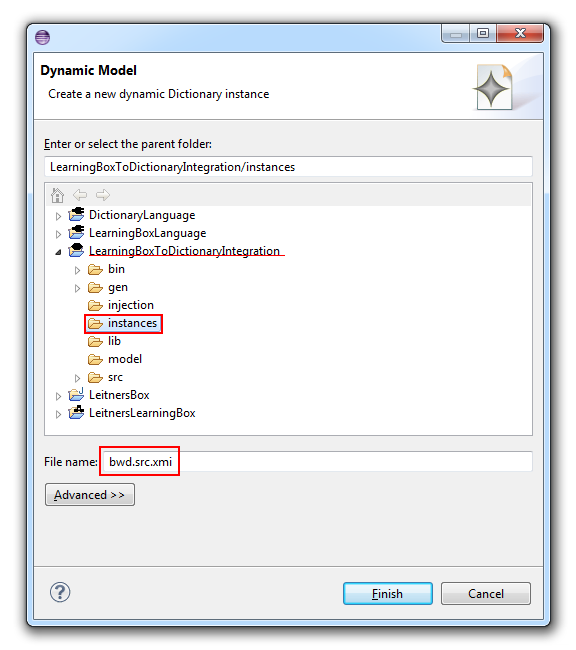
\includegraphics[width=0.8\textwidth]{eclipse_dictionaryInstance}
  \caption{Create a dynamic instance of \texttt{Dictionary}}
  \label{eclipse:create_instance_dict}
\end{center}
\end{figure}

\newpage

\item[$\blacktriangleright$] Open the new file and edit the \texttt{Dictionary} properties by double-clicking and setting \texttt{Title} to \texttt{English
Numbers} in the \texttt{Properties} tab below the window.

\vspace{0.5cm}

\item[$\blacktriangleright$] Create three child \texttt{Entry} objects.
Don't forget the syntax we created for each \texttt{entry.content} in the \texttt{CardToEntryRule} when setting up the constraints! 
Be sure to set this property as \texttt{<word>:<meaning>}. Give each \texttt{entry} a diffirent difficulty \texttt{level}, e.g., \texttt{beginner} for \texttt{One:Eins}, \texttt{advanced} for \texttt{Two:Zwei}, and \texttt{master} for \texttt{Three:Drei}.
Your instance should resemble Fig.~\ref{eclipse:dictionaryxmi}.

\vspace{0.5cm}

\begin{figure}[htbp]
\begin{center}
  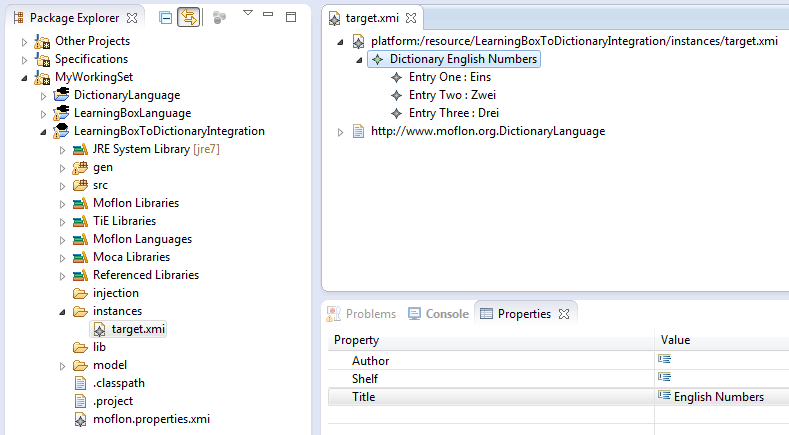
\includegraphics[width=0.75\textwidth]{eclipse_targetThreeEntries}
  \caption{Fill a \texttt{Dictionary} for the transformation}
  \label{eclipse:dictionaryxmi}
\end{center}
\end{figure}

\item[$\blacktriangleright$] Let's check out the file that will actually execute our transformation. Navigate to
``LearningBox\-To\-Dictionary\-In\-te\-gra\-tion\-/\-src/\-org.\-mof\-lon.\-tie'' and click to open
\texttt{Learn\-ing\-Box\-To\-Dict\-ion\-ary\-Int\-e\-grat\-ion\-Trafo.\-java}.

\item[$\blacktriangleright$] As you can see, this file is the driver which runs the complete transformation, first transforming forward from a source
\texttt{box} to a target \texttt{dictionary}, then backward from \texttt{dictionary} to \texttt{box}. As this is plain Java, you can adjust everything freely as
you wish.

\item[$\blacktriangleright$] Right-click the file in the Package Explorer and got to ``Run as\ldots/Java Application'' to execute the file.

\item[$\blacktriangleright$] Did you get one error message, followed by one success message in the eMoflon console window (Fig.~\ref{eclipse:tggERROR}) below
the editor? Perfect! Both of these statements make sense -- our TGG first attempted the forward transformation but, given that it was missing the source
(\texttt{box}) instance, it was only able to perform a transformation in the backwards direction.

\vspace{0.5cm}

\begin{figure}[htbp]
\begin{center}
  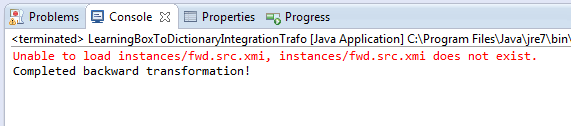
\includegraphics[width=\textwidth]{eclipse_TGGError}
  \caption{Running the backward transformation}
  \label{eclipse:tggERROR}
\end{center}
\end{figure}

\vspace{-0.5cm}

\item[$\blacktriangleright$] Refresh the integration's \texttt{instances} folder. Three new \texttt{.xmi} files should have appeared representing your backward
triple. While you created the \texttt{bwd.src.xmi} instance, the TGG generated \texttt{bwd.corr.xmi}, the correspondence graph between target and source,
\texttt{bwd.protocol.xmi}, a listing of the attempted steps taken (as well as their results), and \texttt{bwd.trg.xmi}, the output of the transformation. Open
this last file in the editor.

\item[$\blacktriangleright$] It's a \texttt{Box} of \texttt{English Numbers}! Expand the tree and you'll see our \texttt{Dictionary} in its equivalent
\texttt{Box} format containing three \texttt{Par\-ti\-tions} (Fig.~\ref{eclipse:derivedBOX}). Double click each \texttt{card} and observe how each
\texttt{entry.content} was successfully split into two sides.

\vspace{0.5cm}

\begin{figure}[htbp]
\begin{center}
  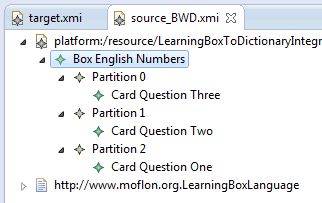
\includegraphics[width=0.5\textwidth]{eclipse_derivedSource}
  \caption{Result of the \emph{backwards} transformation}
  \label{eclipse:derivedBOX}
\end{center}
\end{figure}

\vspace{-0.5cm}

\item[$\blacktriangleright$] Congratulations! You have successfully performed your first \emph{backward} transformation using TGGs!

\newpage

\item[$\blacktriangleright$] Don't forget about one of eMoflon's coolest model visualizing features -- the graph viewer.\footnote{Refer to Part 2, Section 4 to
review how to open and use this tool} This is an especially useful tool for TGGs when you need to quickly confirm your transformation was successful.
Drag-and-drop \texttt{Box English Numbers} into the graph view and open all nodes by double clicking on them (Fig.~\ref{eclipse:graphView}). You should be able to see each \texttt{Card}'s container
\texttt{partition} and the edges via which they'll move between partitions.

\vspace{0.5cm}

\begin{figure}[htb]
\begin{center}
  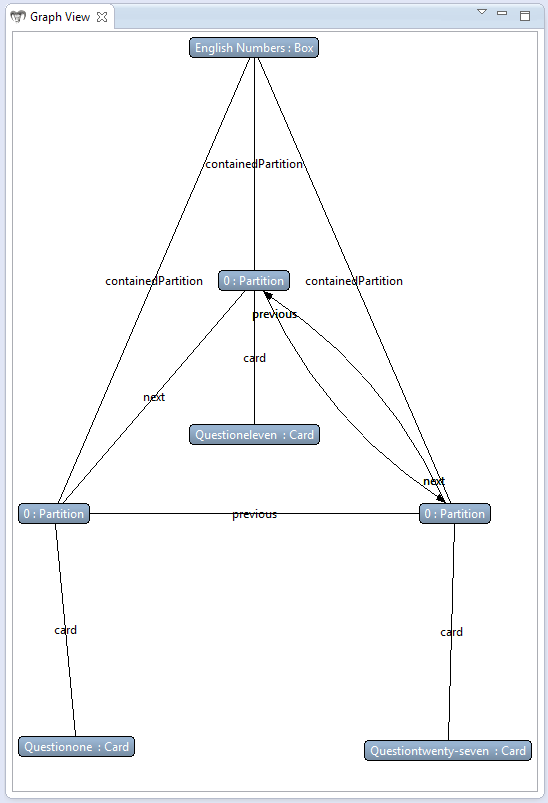
\includegraphics[width=0.6\textwidth]{eclipse_EngNumBoxGraphView}
  \caption{Confirm the transformation with the Graph Viewer}
  \label{eclipse:graphView}
\end{center}
\end{figure}

\vspace{0.5cm}

\item[$\blacktriangleright$] To show that the transformation is actually bidirectional, let's create a source model (thus resolving the error), and run
the TGG again to perform a \emph{forwards} transformation of a \texttt{Box} into a \texttt{Dictionary}. Make a copy of \texttt{bwd.trg.xmi} and rename
it to \texttt{fwd.src.xmi}.

\newpage

\item[$\blacktriangleright$] Run \texttt{LearningBoxToDictionaryIntegrationTrafo} again by pressing the green ``Run As\ldots'' icon on the toolbar. You should
now have two success messages in the console window! Finally, refresh the ``instances" folder and compare the output \texttt{fwd.trg.xmi} against the original
\texttt{bwd.src.xmi} Dictionary model. If everything executed properly, they should look exactly the same.

\end{itemize}
